% File: src/chapter_3_clones.tex
% Project: Monitoring and Reporting Tool for Cloned Vulnerabilities across Open-Source Projects
% Author: Matus Remen (xremen01@stud.fit.vutbr.cz)
% Description: Chapter 3 - Cloned Vulnerabilities

\chapter{Cloned Vulnerabilities}
\label{chapter:clonedVulnerabilities}
Cloned vulnerabilities are weaknesses propagated by reusing source code. This can happen by copy-pasting
insecure code snippets, whole functions or even whole projects. For copying the whole project version control system
Git offers an easy option called a~fork. This allows developers to inherit the infrastructure of an existing project
and afterwards they can modify or start building on it their own features. Although, the inherited code base might
contain vulnerabilities.

In the beginning, this chapter will present an example of a~vulnerability propagated by cloning, followed by
an overview of clone types based on the level of similarity to the origin and methods for their detection. Afterwards,
existing static analysis tools and approaches for the detection of cloned vulnerabilities in the software
will be analysed.

\section{Real-World Example of a~Cloned Vulnerability}
\label{sec:example-cloned-vuln}
  A~notable case of a~flaw propagated by forking or fetching is CVE-2018-17144. On the 18th of September 2018, the bug
  was patched in Bitcoin Core, the primary implementation of the Bitcoin protocol. Besides a~potential Denial of Service (DOS)
  attack, the vulnerability allowed an attacker to double-spend the same input, which would create new bitcoins out of nothing
  and cause inflation in this major cryptocurrency. The flaw was caused by an unhandled assertion error in a~code validating
  transactions and preventing double spending of coins.~\cite{BTCInflationBug, HackerNoonBTCInflationBug}

  \begin{figure}[h]
    \centering
    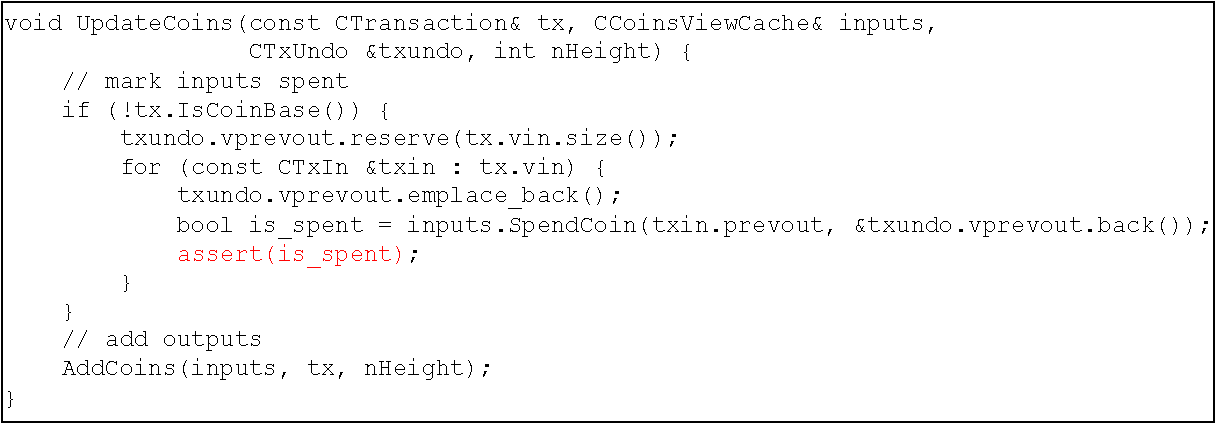
\includegraphics[width=0.9\textwidth]{obrazky-figures/cve-2018-17144_code.drawio.pdf}
    \caption{Vulnerable code shared between Bitcoin and PigeonCoin. Source:~\cite{BTCInflationBug}}
    \label{cve201817144code}
  \end{figure}

  The bug was fixed in Bitcoin Core before it could have been exploited. Unfortunately, in the case of PigeonCoin,
  one of many forks of Bitcoin, attackers took advantage and generated 235~million coins worth of around 15,000 USD
  on 26th of September 2018, while it was still vulnerable more than a~week after the fix in Bitcoin Core.
  The propagated code responsible for the vulnerability is visible in Figure~\ref{cve201817144code}.~\cite{CoinDeskPGNInflationBug,
  HackerNoonBTCInflationBug}
  % TODO 2 more

\section{Types of Code Clones}
  Clones of source code originate from copying and reusing code fragments with possible modification
  is a~common approach in software development. Such activity is an efficient way in programming as similar
  code does not have to be written multiple times from scratch. Depending on how similar the code clones are to
  their origins, they are divided into four groups~\cite{CodeClonesSurvey}. For an example of each type of clone
  consider the following code in the programming language C as the original code:
  \begin{alltt}
  if (a > b) \{  // comment
      a = b + 1;
  \} else \{
      a = b + c;
  \}
  \end{alltt}
  \textbf{Type~I} clones are identical code fragments with possible white space characters and comment
  variations.
  Type~I clone from the example original code could be:
  \begin{alltt}
  if (a > b) \{
      a = b + 1; \textcolor{red}{\}  // comment 1}
  else \{
      a = b + c; \textcolor{red}{\}  // comment 2}
  \end{alltt}
  \textbf{Type~II} are Type~I clones with additional possible variations in user-defined identifier naming
  and types. An example could be:
  \begin{alltt}
  if (\textcolor{red}{x} > \textcolor{red}{y}) \{
      \textcolor{red}{x} = \textcolor{red}{y} + 1;  \textcolor{red}{// comment}
  \}
  else \{ \textcolor{red}{x} = \textcolor{red}{y} + \textcolor{red}{z}; \textcolor{red}{\}}
  \end{alltt}
  \textbf{Type~III} clones in addition to Type~I and Type~II contain changed, added and/or deleted statements.
  Type~III clone might look like this:
  \begin{alltt}
  if (x > y) \{
      x = y + 1;
  \} else \{  // comment
      \textcolor{red}{flag = 1;  // addition}
      x = y + z;
  \}
  \end{alltt}
  \textbf{Type~IV} are code fragments with different syntactical structures, but with the same semantics. Unlike
  the previous types which were textually similar, this type of clone is defined by functional similarity.
  An example of a~Type~IV clone might look accordingly:
  \begin{verbatim}
  x = x > y ? y + 1 : y + z;
  \end{verbatim}

\section{Detection Methods}
  Detection techniques are divided into four classes: textual, lexical, syntactic and semantical.
  This section will introduce each class and mention detection tools which are based on them.

  \subsubsection*{Textual Approaches}\label{clone-detection:simian}
    Text-based approaches compare two code fragments and detect clones based on string comparison of lines.
    They are language-independent, easy to implement and generate fewer false positive results. Before detection,
    they tend to use normalization like the removal of white spaces and comments. This approach is able to detect
    Type~I clones without further post processing~\cite{CloneDetectionTechniques, CodeClonesSurvey}. Tools which
    are based on this approach include Dup~\cite{Dup} and NICAD~\cite{NICAD}.

  \subsubsection*{Lexical Approaches}
    In lexical or token-based approaches whole source code of the analysed project(s) is parsed into a~sequence
    of tokens. Then in the next step, the generated sequence of tokens is scanned for duplicate subsequences which
    represent code clones in the end. CCFinder~\cite{CCFinder} and CPMiner~\cite{CPMiner} are example tools
    utilizing this approach. They are able to detect clones of various types and have higher precision than
    textual approaches, but they also have some limitations. These techniques have higher time and space
    complexity and are dependent on the order of the tokens and lines. When cloned code contains added or deleted
    tokens, this approach will not detect it as clone~\cite{CloneDetectionTechniques, CodeClonesSurvey}.

  \subsubsection*{Syntactic Approaches}
    Syntactic approaches contain two types of techniques -- tree-based and metric-based.

    Tree-based approach parses the source code of the analysed project firstly into tokens which are used
    to build an abstract syntax tree (AST). Then the clones are detected using tree-matching algorithms rather
    than matching sequences of tokens in lines as in lexical approaches. In this case, similar sub-trees
    represent duplicate code. Tools developed by Baxter et al.~\cite{ASTBaxter} and by Wahler et
    al.~\cite{ASTWahler} implement the tree-based approach.

    The second type, the metric-based approach uses a~number of different metrics gathered from syntactic units
    like classes, methods, functions or statements in the target source code. The metric vectors are then compared
    in order to detect clones instead of searching through AST or comparing code directly. Some of the collected
    metrics in tools implementing this approach can be numbers of loop, conditional and return
    statements~\cite{CloneDetectionTechniques, CodeClonesSurvey}.
    Implementations of metric-based approach are for example tools developed by Mayrand et al.~\cite{MBMayrand}
    or by Abdul-El-Hafiz et al.~\cite{MDAbdul}.

  \subsubsection*{Semantic Approaches}
    This type of approach is used to detect code fragments with similar semantics but different code structures.
    There are two approaches connected with this technique -- graph-based and hybrid.

    The graph-based approach utilizes a~Program Dependency Graph (PDG) to represent data and control
    the flow of the analysed source code. The detection is performed by an isomorphic subgraph matching algorithm.
    For example, tool GPLAG~\cite{GPLAG} implements this approach.

    The hybrid detection technique combines multiple approaches which were mentioned
    above~\cite{CloneDetectionTechniques, CodeClonesSurvey}. An approach developed by Agrawal et
    al.~\cite{HybridAgrawal} uses this technique.

\section{Detection Tools}
Detection tools and approaches analysed in this section are tools designed for the automatic identification of
security vulnerabilities in software applications. Common types are static analysis tools,
dynamic analysis tools and penetration testing tools. Static analysis tools scan software source code
to identify potential weaknesses, while dynamic analysis tools observe the behaviour of the system during
run-time. Penetration testing tools are designed to simulate attacks on the system to identify
vulnerabilities, which might be exploited during a~cyberattack.

  \subsection*{CoinWatch}
    \textit{This subsection is based on~\cite{CoinWatch}.}
    CoinWatch is a~static analysis tool utilizing a~clone-based approach for detecting vulnerabilities
    in cryptocurrencies. Cryptocurrencies are an attractive commodity for attackers because they can be
    anonymously sold on exchanges. The fact, that many of them have their source code publicly available,
    makes it possible to develop tools like CoinWatch. It was developed in 2020 and has achieved promising
    results, but unfortunately, it is not available for public use.

    In summary, CoinWatch reported 786 vulnerabilities in 384 cryptocurrencies to the date, when the paper
    was written and achieved a~true positive rate of 89.7\%. To the date, CoinWatch worked only with Type~I
    clones, while Type~II and Type~III would need a~more sophisticated method of detection like analysis of
    decompiled binaries of projects. In future work, creators want to investigate possibilities for how to
    detect also Type~II and Type~III clones alongside automating the process of the manual code
    annotation.

    A~study connected with CoinWatch contains an analysis of the propagation of cloned source code between
    cryptocurrencies. The analysis found that at the time 786 cryptocurrencies were directly or indirectly
    cloned from a~version of Bitcoin. The percentage of cloned code in projects forked from Bitcoin
    is displayed in Figure \ref{bitcoin-clone-ratio}. In the majority of these projects, the clone ratio was
    below 30\%, however, some had the ratio even higher than 50\%. This fact implies the potential propagation
    of vulnerabilities among clones, once they are discovered in the parent project. In the case of
    cryptocurrencies, neglecting the maintenance of the adopted code may have a~serious financial impact.
    Also, the number of detected projects by the analysis is high, which makes maintenance a~very costly
    and repetitive task. CoinWatch is a solution for filtering only potentially vulnerable projects,
    whose maintainers can be accordingly warned about the detected threat.

    \begin{figure}[h]
      \centering
      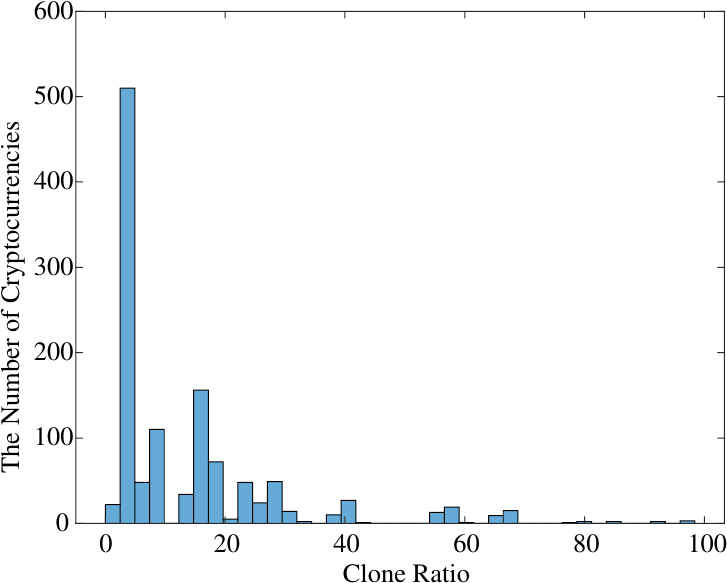
\includegraphics[width=0.5\textwidth]{obrazky-figures/clone_ratio_histogram.png}
      \caption{Bitcoin v0.17.0 clone ratio in forked projects. Source:~\cite{CoinWatch}}
      \label{bitcoin-clone-ratio}
    \end{figure}

    The overall workflow of CoinWatch is visualized in Figure~\ref{coinwatch-workflow}. At the beginning
    of the pipeline, the tool receives a~target CVE assigned to the target project. Accordingly, all publicly
    available details about the desired vulnerability are scraped and parsed from vulnerability databases.
    These details are input for the next step -- code evolution analysis. The analysis utilizes the version
    control system Git for traversing the versions of the target project. Using the parsed CVE details,
    the analysis aims to identify fixing and bug-introducing commits for the provided vulnerability
    in the repository of the project. Identified fixing and bug-introducing commits create a~time window, in which
    the target project was affected by the vulnerability. This time window is used for the initial filtering
    of potentially affected child projects, which were forked from the target project during this period.
    The identified fixing and bug-introducing commits are additionally used for manual annotation of
    the vulnerable code and transformation to a~clone detection pattern. In the end, the clone detection tool
    checks the occurrence of the pattern in the potentially vulnerable projects forked in the time window.
    After clone detection, on the output of the pipeline is a~list of likely affected cryptocurrencies.

    \begin{figure}[h]
      \centering
      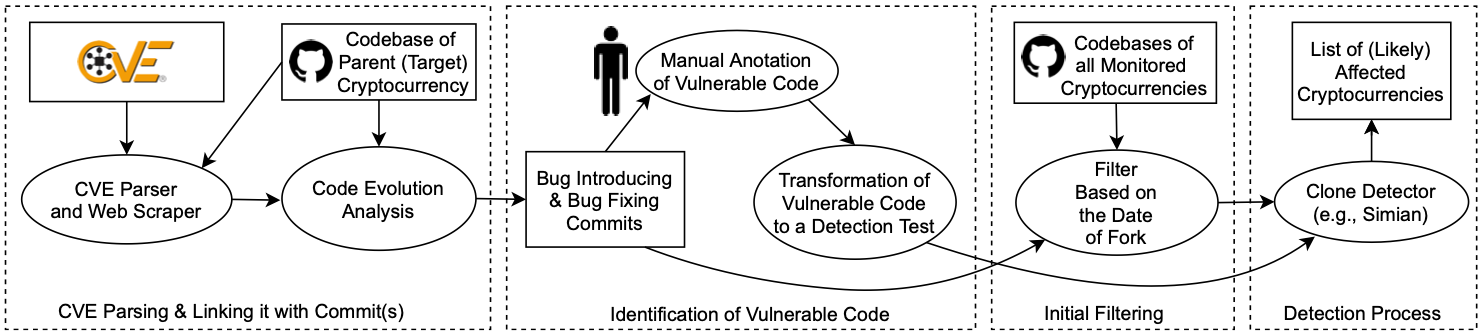
\includegraphics[width=1\textwidth]{obrazky-figures/coinwatch_workflow.png}
      \caption{Overall workflow of tool CoinWatch. Source:~\cite{CoinWatch}}
      \label{coinwatch-workflow}
    \end{figure}

    \subsubsection*{CVE Parsing and Linking with Commits}
      In this step, CoinWatch scrapes and parses details of the selected vulnerability. Following data
      is extracted from details about CVE in vulnerability databases:
      \begin{itemize}
          \item date of publishing
          \item keywords from description
          \item references pointing to the version control system of the affected project
          \item the list of affected cryptocurrencies and their programming language
      \end{itemize}
      After parsing, the origin of the vulnerability is checked, and whether the issue is connected with specific
      code as the threat may originate from using outdated versions of libraries, frameworks and protocols.
      In case of code-specific weakness, the code evolution analysis links patching and bug-introducing
      commits with the CVE.

    \subsubsection*{Code Evolution Analysis -- SZZ Algorithm}
    For the purpose of code evolution analysis, CoinWatch utilizes the SZZ algorithm. The algorithm was proposed
    by Sliwerski, Zimmermann and Zeller~\cite{SZZalgorithm} as an approach for identifying bug-introducing
    commits. An open implementation of the algorithm is named SZZ Unleashed~\cite{SZZunleashed}. It is written
    in Java programming language with supporting Python scripts. SZZ Unleashed works in two phases. The first
    phase identifies bug-fixing commits used in the second phase for tracking the bug-introducing changes.
    CoinWatch is built on this algorithm and extended it for the tool's specific purposes.

    Firstly, using parsed details about the vulnerability, the bug-fixing commits are identified from
    the version control system in the affected project. In CoinWatch this is done by matching regular expressions
    in issues which have been fixed, resolved, closed or labelled as ``bug''. The regular expression is built
    from keywords extracted from the description in CVE details and keywords ``CVE'' and ``CVE-ID''.

    Secondly, for each discovered fixing commit the bug-introducing commits are tracked utilizing the second
    phase of the SZZ algorithm. This phase leverages the command git-blame and line number mapping to backtrack
    through the history of the analysed project. This method maps only the lines affected by the
    analysed commit as shown in Figure \ref{szz-line-map}. In addition, this phase provides an option to
    select the desired depth of mapping the line numbers over a~variable number of versions, indicated by
    the depth parameter. In the provided example, working with the depth option set to one would result in
    not identifying the bug introduced by Commit 2, because it is in depth two and it is detectable only from
    the annotation of commits 3, 4 and 5.

    \subsubsection*{Identification of Vulnerable Code and Initial Filtering}
    Inputs for this part of the CoinWatch are bug-fixing and their matching bug-introducing commits.
    For initial filtering of potentially vulnerable forks, CoinWatch selects the newest bug-fixing commit
    and the oldest bug-introducing commit to form a~time window. Monitored forked projects are then filtered
    based on the timestamp of their fork. When it is within the time window they are marked as potentially
    vulnerable candidates. The projects around the time window are ignored.

    Identification of vulnerable code is a~one-time manual process per CVE. The goal of this step is to
    extract the patch code and the vulnerable code from commits detected during code evolution analysis.
    After the manual code annotation, it is transformed into a~detection test as input for the clone detection
    tool.

    \begin{figure}[h]
      \centering
      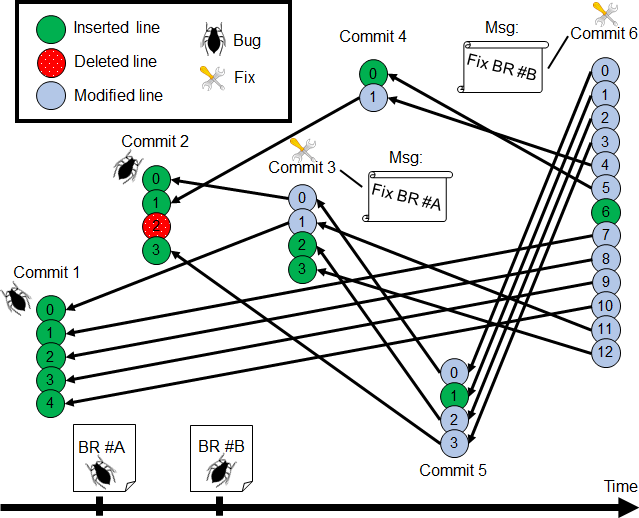
\includegraphics[width=0.7\textwidth]{obrazky-figures/szz_line_mapping.png}
      \caption{An example of SZZ Unleashed mapping line numbers. Source:~\cite{SZZunleashed}}
      \label{szz-line-map}
    \end{figure}

    \subsubsection*{Clone Detection Process}
    Finally, CoinWatch triggers the clone detection tool Simian \ref{clone-detection:simian} with the detection
    test on the list of potentially vulnerable candidates from the previous step. This filters the projects
    that already patched the vulnerability or reimplemented the part of code, which was vulnerable in the
    source project and returns the final list of likely vulnerable projects.

  \subsection*{BlockScope}
  \label{section:blockscope}
    \textit{This subsection is based on~\cite{BlockScope}.}
    BlockScope is a~novel tool for detecting vulnerabilities propagated by cloning blockchain projects like
    Bitcoin and Ethereum. It is a~language-agnostic tool capable of detecting multiple vulnerabilities from
    existing security patches. BlockScope utilizes similarity-based code match and designs
    a~new way of calculating code similarity. Thanks to this approach it is able to detect Type~I, Type~II and
    Type~III clones. Additionally, it is capable of automatic extraction of security patch contexts in comparison
    to CoinWatch.

    Figure \ref{blockscopeworkflow} presents the overall workflow of BlockScope. Initially,
    the tool receives a~security patch and the affected project on the input. The security patch is accepted
    either in the form of a~commit ID from the source project or manually crafted patch contexts for better accuracy.
    A~patch context represents a~surrounding of the code changes in the patch commit. The component named
    Extractor serves for identifying patch context when the commit ID of the security patch is provided.
    Subsequently, the component Searcher tries to match the patch context in the analysed project which produces
    a~candidate context. Then Fetcher uses the contexts to extract patch code from the source project
    and potentially vulnerable candidate code from the target project. The similarity of the extracted
    codes is then measured in Comparator, which determines whether the target project was patched. Additionally,
    for the vulnerabilities that were already fixed in the target repository, BlockScope performs
    the calculation of patch delay.
    \bigskip
    \begin{figure}[h]
      \centering
      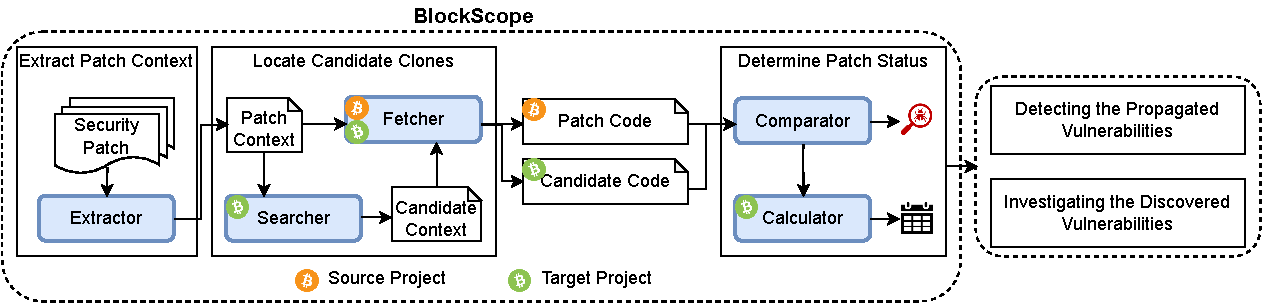
\includegraphics[width=0.99\textwidth]{obrazky-figures/blockscope_workflow.pdf}
      \caption{Overall workflow of tool BlockScope. Source:~\cite{BlockScope}}
      \label{blockscopeworkflow}
    \end{figure}

    BlockScope achieved overall precision and recall both at the rate of 91.8\%. It discovered 101 previously
    unknown vulnerabilities propagated via code cloning in 13 out of 16 analysed projects forked from Bitcoin
    and Ethereum. Unfortunately, just like CoinWatch it is not available for public use and is
    close sourced.

    \subsubsection*{Patch Context Extraction}
    The initial step of BlockScope extracts the context of the given security patch on the input. The patch context
    consists of two components -- upper and lower. The extraction is depicted in Figure~\ref{figure:blockscope-search}
    on a~patch code on the left side and the process is following.

    Firstly, the code surrounding the patch is tokenized. Tokenization considers both upper and lower case characters
    and additionally includes some special characters such as ``.'' and~``!''. Then, in each context line, the longest
    token is selected as a~keyword representing the sentence. The keywords together identify the patch context in the next
    step in the processing. In the example displayed in Figure~\ref{figure:blockscope-search}, the selected keywords
    are marked by a~red font colour.

    \subsubsection*{Localization of Candidate Code Clones}
    In this step, BlockScope searches for all candidate code clones in target repositories using components Searcher and Fetcher.
    Figure~\ref{figure:blockscope-search} illustrates this process on patch commit \texttt{0e7c52dc} in Bitcoin
    and a~cloned code chunk present in Dogecoin, a~fork of Bitcoin.

    The localization begins with selecting key statements from each patch context in the target repository.
    To determine key statements, the component Searcher firstly utilizes a~command \texttt{git grep} to find
    all code statements containing the patch keywords extracted in the previous step. Finally,
    each found code statement is compared to the original code statement in the patch context and the most similar
    one is selected as a~key statement in each context.
    For calculating the similarity, BlockScope uses the Normalized Levenshtein edit distance metric with a~threshold
    equal to 0.25.

    The threshold is used to minimize misses and avoid false negative results in the rest of the workflow.
    In the current step, the threshold is used to filter code statements with low similarity to the original
    statement. Additionally, the tool uses here three other optimizations. The first excludes comments and test code
    from keyword search results. The second filters search results based on the type of file affected by a~patch
    and the third checks the type of code statements.

    Once the key statements are identified, the goal of the next step is to extend the single statement to multi-line
    candidate context. This is done by extracting the surrounding code around the key statement until the candidate
    context contains the same number of lines as the patch context, which is specified by a~constant \texttt{C\_LINES}.
    Then, the boundary is determined by comparing each line in the candidate context to the start and end statements.
    In the end, just like in the case of the key statement, the start and end statements in the candidate context are specified
    by the highest similarity exceeding the threshold.

    Finally, the candidate contexts are yet compared to the patch using the same evaluation method as used for
    determination of patch application status~\ref{similarity-equation}.
    Candidate contexts with similarity below the threshold are discarded and the others are forwarded to the component
    Fetcher. As for the patch, so for candidate contexts, the component Fetcher extracts the code between the upper and lower
    context, returning a~patch code and a~list of candidate codes for further analysis.

    \begin{figure}[h]
      \centering
      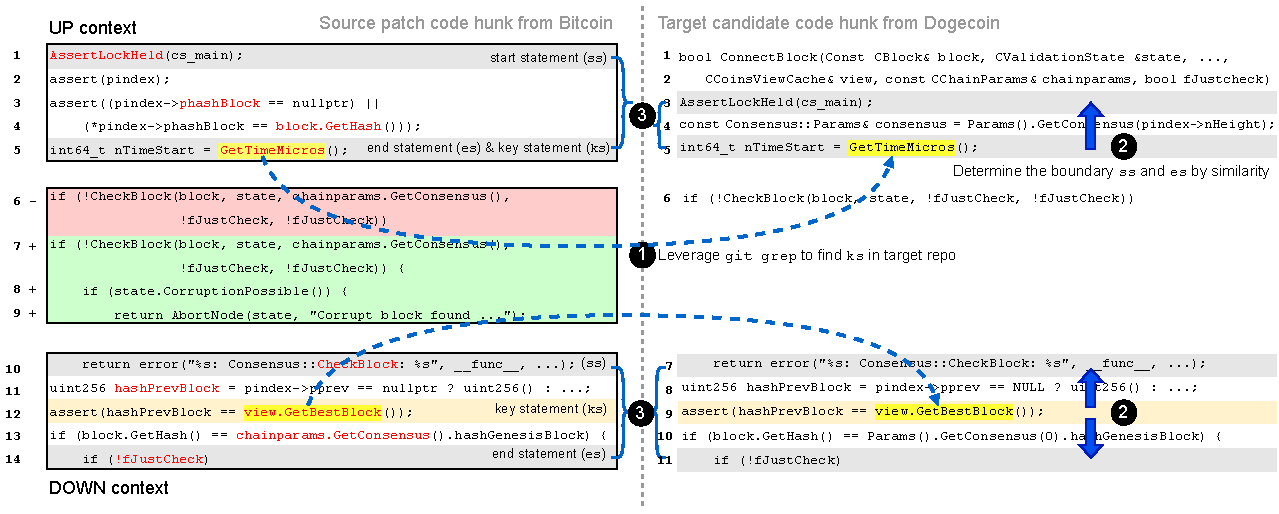
\includegraphics[width=1\textwidth]{obrazky-figures/blockscope_search.drawio.pdf}
      \caption{Visualization of context-based search of BlockScope for searching candidate contexts in a~target repository.
       Source:~\cite{BlockScope}}
      \label{figure:blockscope-search}
    \end{figure}

    \subsubsection*{Determination of Patch Status}
    The last step of the workflow, the determination of the patch application status is performed in components Comparator
    and Calculator. The Comparator measures the similarity between the patch and each candidate and evaluates, whether
    the target project applied the patch, hence whether it is vulnerable or did not inherit that particular part
    of the code. The projects, which applied the patch are further analysed by the component Calculator, which
    calculates a~patch delay.

    BlockScope designs a~new way of measuring the similarity between two code fragments, which is capable of detecting
    the first three types of clones. The way is shown in the following Equation~\ref{similarity-equation}, where
    $S$ stands for source and $T$ for target code fragment with $p$ and $q$ code statements. The similarity measure
    is defined as the weighted average of the similarity of each sentence from $S$ and its most similar pair among $T$.
    The function $strsim$ calculates the Normalized Levenshtein distance metric~\cite{strsim} of two strings, which returns a~value
    in the interval $[0, 1]$. To cover clones of Type~III, as they contain inserted, deleted and reordered statements,
    this way introduces parameter $r \in [0, 1]$ and $r^{\vert i-j \vert}$ to specify the reward of the similarity result
    between $S_i$ and $T_j$.

    \begin{equation}
      \begin{aligned}
        \text{SIMILARITY}(S, T)\ &=& \frac{1}{p} \sum \limits^p_{i=1}\text{strsim}(S_i, T_j)r^{\vert i-j \vert} \\
        \text{s.t. } j\ &=& \mathop{arg\ max\ }_{1 \leq k \leq q} \text{strsim}(S_i, T_k)
        \label{similarity-equation}
      \end{aligned}
    \end{equation}

    To determine whether a~patch ($P$) was applied, it is compared to the candidate code ($C$) and BlockScope uses three
    rules for that evaluation. There are three possible types of patches. One which contains only code additions (\texttt{ADD} type,
    $P = [ap]$), a~one with code deletions only (\texttt{DEL} type, $P = [dp]$) and the third, which contains both
    (\texttt{CHA} type, $P = [ap, dp]$). Using the described similarity measure, each type has its own definition of applied status.
    Consider variables $sa = SIMILARITY(C, ap)$ and $sd = SIMILARITY(C, dp)$ for better readability in the following description
    of the rules for each type.
    \begin{itemize}
        \item \texttt{ADD} type: if $sa \geq t$, it is evaluated, that $P$ was applied in $C$, else it was not.
        \item \texttt{DEL} type: if $sd \geq t$, it is evaluated, that $P$ was not applied in $C$, else it was.
        \item \texttt{CHA} type: if $sd \geq t$ and $sa \geq t$ and $sd \geq sa$, it is evaluated that $C$ did not apply $P$,
              otherwise if $sd \geq t$ and $sa \geq t$ and $sd < sa$, it is evaluated that $C$ applied $P$
    \end{itemize}

    The components from the previous step can return more than one candidate context, and so produce multiple candidate
    code fragments $C_i \in [C_1, C_2, ..., C_n]$. In this case, similarity of each candidate, $s_i = SIMILARITY(C_i, P)$,
    and its patch application status, $fv_i \in \{0, 1\}$, is calculated, where $f_i = 1$ indicated, that $C_i$ applied patch $P$.
    To finalize the results, factor $conf_i = s_i - t$ is introduced to measure the confidence of each result. In the end,
    the result with highest confidence $fv_i$, where $i = arg\ max_j\ conf_j$, is selected as the final result of application
    status.

    Projects, which already applied the patch are additionally analysed by component Calculator. Calculator leverages
    command \texttt{git blame} to extract the hash of the commit, which patched the vulnerability in the target repository.
    The command returns additionally to each line of code in the provided file the latest commit, which changed the line.
    Using this information, the commits on the lines of candidate code are fetched. If the candidate code was changed
    by multiple commits, the earliest one is considered as fixing. In the end, the component Calculator calculates
    the delay between the patch commit in the original repository and the extracted commit in the target repository.

% https://www.researchgate.net/publication/335152710_Detecting_Security_Vulnerabilities_using_Clone_Detection_and_Community_Knowledge
